%%%%%%%%%%%%%%%%
% Class
%%%%%%%%%%%%%%%%

	\documentclass[twoside]{article}
	
%%%%%%%%%%%%%%%%
% Packages
%%%%%%%%%%%%%%%%

	\usepackage[margin=1in]{geometry}
	\usepackage{graphicx}
	\usepackage{amsmath}
	\usepackage{tikz}
		\usetikzlibrary{shapes}
%		\usetikzlibrary{decorations}
%		\usetikzlibrary{decorations.pathreplacing}
%		\usetikzlibrary{decorations.pathmorphing}
	\usepackage{fancyhdr}

%%%%%%%%%%%%%%%%
% Other opts and styling
%%%%%%%%%%%%%%%%

	\graphicspath{{./assets/}}
	
	% Page headers
	\fancypagestyle{style1}{
		\renewcommand{\headrulewidth}{0pt}
		\fancyhead{}
		\fancyhead[LE,RO]{\bfseries McDonald Lab Standard Operating Procedures}
		\fancyhead[LO,RE]{\thepage}
		\fancyfoot{}
	}
	
	\fancypagestyle{style2}{
		\renewcommand{\headrulewidth}{0pt}
		\fancyhead{}
		\fancyhead[LE,RO]{\bfseries McDonald Lab Daily Log}
		\fancyhead[LO,RE]{\thepage}
		\fancyfoot{}
	}
	
%%%%%%%%%%%%%%%%
% BEGIN DOCUMENT
%%%%%%%%%%%%%%%%

	\begin{document}

%%%%%%%%%%%%%%%%
% New commands
%%%%%%%%%%%%%%%%
	
	% Thick horizontal rule
	\newcommand{\HRule}{\rule{\linewidth}{0.5mm}}
	
	% Easy scientific notation
	\newcommand{\e}[1]{\ensuremath{\times 10^{#1}}}

%%%%%%%%%%%%%%%%
% TITLE PAGE
%%%%%%%%%%%%%%%%
	\pagestyle{style1}
	%!TEX root=./labNotes.tex

\begin{titlepage}
	{~ \\[5cm] }
	
	\noindent \HRule \\[0.4cm]
	{ \Huge \bfseries McDonald Lab \\[0.4cm] }
	{ \huge \bfseries Lab Protocols and Daily Log \\ }
	\HRule \\[0.4cm]
	
	\noindent { \Large Christopher Wetherill \\[0.15cm] }
	{ \large \emph{Virginia Polytechnic Institute and State University} }\\[11cm]
	
	\noindent Audit log available at https://github.com/faulconbridge/TBMH/tree/master/Virology
\end{titlepage}
	\setcounter{page}{1}
	
%%%%%%%%%%%%%%%%
% CONTENTS
%%%%%%%%%%%%%%%%

	\part{Standard Operating Procedures}
	%%%%%%%%%%
	% Protocol
	%%%%%%%%%%
	%!TEX root=./virology.tex

\section{Lab Protocols}

\subsection{Location of Common Materials}

\begin{tabular*}{\textwidth}{r | p{2in} p{2in}}
\hline
Item & Location & Storage \\
\hline
(In)complete Medium 199 & Incomplete Medium 199 is located in the cold room in the hallway immediately outside the lab. & Complete and serum-free Medium 199s are stored in the $4^{\circ}$C freezer in R2048.\\
Penicillin/Streptomycin Stock & P/S stock is located in the $-20^{\circ}$C freezer in the hallway immediately outside the lab. & Leftover stock is stored in the $4^{\circ}$C freezer in R2048.\\
L-Glutamine Stock & Stock is located in the $-20^{\circ}$C freezer in the hallway immediately outside the lab. & Leftover stock is stored in the $4^{\circ}$C freezer in R2048.\\
Amphotericin B stock & Stock is located in the $-20^{\circ}$C freezer in the hallway immediately outside the lab. & Leftover stock is stored in the $4^{\circ}$C freezer in R2048.\\
0.05\% Trypsin-EDTA & Stock is located in the $-20^{\circ}$C freezer in the hallway immediately outside the lab. & Leftover stock is stored in the $4^{\circ}$C freezer in R2048.\\
Trypsin ($2$mg/mL) & Stock is located in the $-20^{\circ}$ freezer in the hallway immediately outside the lab. & Leftover stock should be refrozen in a box labelled with your name.\\
Fetal Bovine Serum & Stock is located in the $-20^{\circ}$C freezer in the hallway immediately outside the lab. & Leftover stock is stored in the $4^{\circ}$C freezer in R2048.\\
(In)complete 2x EMEM & Stock is located in the cold room in the hallway immediately outside the lab. & Complete EMEM stock is stored in the $4^{\circ}$C freezer in R2048.\\
SeaPlaque Agarose & Stock is located in a jar above the benches immediately outside of the biosafety cabinet. & Leftover stock should be replaced where you found it.\\
10x PBS & Stock is located in a plastic bottle above the benches immediately outside of the biosafety cabinet. & Leftover stock should be replaced where you found it. \\
SA11 Stock & Stock is located in the $-20^{\circ}$ freezer in the hallway immediately outside the lab. & Leftover stock should be replaced where you found it.\\
Natural Red & Stock is located in the $4^{\circ}$ freezer in R2048. & Leftover stock should be replaced where you found it.\\
Lentiviral stock & Stock is located at the $-80^{\circ}$C freezer in the hallway immediately outside the lab. & Leftover stock should be replaced where you found it. \\
Polybreen & Stock is located in the $-20^{\circ}$C freezer in the hallway immediately outside the lab. & Leftover stock should be returned where you found it.\\
\hline
\end{tabular*}

\subsection{Recording Work and Labelling Materials}

All solutions should be labeled with your name, the date of preparation, and what the solution contains. All cell flasks should be labeled with your name, the date of preparation, the type of cell contained, and the passage of cell contained.

All work completed in the lab should be recorded in a laboratory notebook. Each page should contain entries from only a single day. The date of entry should be recorded at the top of each page. All writing must be easily readable and written in pen. Any errors should be struck through with a single solid line with the correction appearing next to it. Any space on a page not used at the end of a work day should be clearly crossed out in pen.

\subsection{Procedures for Autoclaving}

Ensure that all items have autoclave tape (if necessary). Place all items into the plastic bin found on the cart next to R2048. Take to the autoclave room. Add an autoclave quality indicator strip to the bin and insert into the autoclave. Close the door and select the appropriate options based on what is being sterilized. Start the cycle and fill out the autoclave use form on the bench next to the machine. Once the cycle is complete, retrieve the bin using the thick insulated gloves found in the lab (next to where the bin is stored). It is normal for there to be a small amount of water in the base of the bin.

\subsection{Preparation of Medium 199 (Serum-Free)}

{\bfseries Items Needed:}\footnote{The paper {\itshape Culturing, Storage, and Quantification of Rotaviruses} advises using different quantities of some materials below. Nonetheless, the following are the recommended quantities for use in lab.} \begin{enumerate}
	\item Incomplete Medium 199 ($500$mL)
	\item Penicillin/streptomycin stock ($5$mL)
	\item Amphotericin B stock ($1$mL; $250\mu$g/mL)
\end{enumerate}

In the biosafety cabinet, supplement $500$mL incomplete Medium 199 with $5$mL P/S stock and $1$mL amphotericin B stock. Store at $4^{\circ}$C for up to 3 months.

\subsection{Preparation of Medium 199 (Complete)}

{\bfseries Items Needed:}\footnote{See Note 1.} \begin{enumerate}
	\item Incomplete Medium 199 ($500$mL)
	\item Penicillin/streptomycin stock ($5$mL)
	\item Amphotericin B stock ($1$mL; $250\mu$g/mL)
	\item Fetal bovine serum ($55$mL)
\end{enumerate}

In the biosafety cabinet, supplement $500$mL incomplete Medium 199 with $5$mL P/S stock, $1$mL amphotericin B stock, and $55$mL fetal bovine serum. Store at $4^{\circ}$C for up to 3 months.

\subsection{Preparation of 1.2\% Agarose}

{\bfseries Items Needed:} \begin{enumerate}
	\item SeaPlaque agarose
	\item Milli-Q filtered water
\end{enumerate}

To a $500$mL flask add $1.2$g agarose for every $100$mL water. Inadvisable to fill flask to more than $400$mL. Cap and shake. Loosen lid. Apply autoclave tape to the lid. Autoclave approx. 20 min.

\subsection{Preparation of 2x EMEM (Serum-Free)}

{\bfseries Items Needed:} \begin{enumerate}
	\item incomplete 2x EMEM ($500$mL)
	\item $200$mM \textsc{l}-glutamine ($10$mL)
	\item P/S stock ($10$mL)
	\item $250\mu$g/ml amphotericin B stock ($1$mL)
\end{enumerate}

In the biosafety cabinet, to $500$mL incomplete 2x EMEM stock add $10$mL \textsc{L}-glutamine, $10$mL P/S stock, and $1$mL amphotericin B stock. Store at $4^{\circ}$C for up to 3 months.

\subsection{Preparation of PBS (Phosphate Buffered Saline)}

{\bfseries Items Needed:} \begin{enumerate}
	\item 10x PBS ($80$mL)
	\item milli-Q water ($720$mL)
\end{enumerate}

To a large graduated cylinder add $80$mL 10x PBS solution (use a $25$mL pipet). Fill the graduated cylinder to $800$mL with milli-Q-filtered water. Apply autoclave tape to the lid. Autoclave for 30 minutes.

\subsection{Procedure for Splitting MA104 Cells}

{\bfseries Items Needed:} \begin{enumerate}
	\item 1x PBS
	\item 0.05\% Trypsin-EDTA
	\item Complete Medium 199
	\item $150$cm$^2$ flask
\end{enumerate}

In a water bath, warm PBS, Trypsin, and complete Medium 199 to $37^{\circ}$C. Transfer all materials into the biosafety cabinet. Tilt the flask with your cells (having formed a confluent monolayer) such that the culture medium runs towards the neck of the flask. Vacuum out all culture medium using a small glass pipet inserted into the rubber vacuum hose. Dispose of the pipet. To the cell culture, add 10mL 1x PBS. Tilt the flask to ensure that all cells are thoroughly covered by PBS. Aspirate using a small glass pipet. Dispose of the pipet.

To the cell culture, add $5$mL Trypsin, tilting the flask forward and back to ensure that the cells are fully bathed. Vacuum out the Trypsin with a small glass pipet. Add a second $5$mL portion of Trypsin to the cell culture. Incubate at $37^{\circ}$C until all cells have detached from the surface and are free-floating. Lightly tap the flask with your hand if any cells remain attached.

To the cell culture add $15$mL complete Medium 199. (If you used less trypsin in the previous step, adjust the amount of Medium 199 applied such that there is $20$mL solution in the flask.)

To each new flask that you wish to prepare, add complete Medium 199 such that the final flask volume after the cell mixture is added will be equal to $25$mL. To determine the volume of cell mixture to add to each new flask, we use Table 1.1.

\begin{figure}[htp]
{\bfseries Table 1.1}\\[0.1cm]
\begin{tabular*}{\textwidth}{c c}
\hline
Cell dilution ratio & Cell mix volume to add \\
\hline
1:2 & 10mL \\
1:4 & 5mL \\
1:8 & 2.5mL \\
\hline
\end{tabular*}\\[0.1cm]
{\small {\itshape Note.} For example, if we wished to prepare one 1:4 dilution and two 1:8 dilutions, to our first flask we would add $15$mL complete Medium 199 and 10mL cell mixture; to each of our second two flasks we would add $20$mL complete Medium 199 and $5$mL cell mixture.}
\end{figure}

Cap the new flask(s) and tilt forward and back to evenly spread the cells. Loosen the lids and incubate at $37^{\circ}$C.

\subsection{Procedure for Plating MA104 Cells}

{\bfseries Items Needed:} \begin{enumerate}
	\item 1x PBS
	\item 0.05\% Trypsin
	\item Complete Medium 199
	\item Trypan Blue
	\item 6-well plates (x4)
\end{enumerate}

Aspirate the cell culture medium from the flask. Wash the cell monolayer in $10$mL $1x$ PBS and aspirate from the flask. Wash the cell monolayer in 5mL trypsin and aspirate from the flask. Bathe the cell monolayer in 5mL trypsin and incubate at $37^{\circ}$C until all cells have detached from the flask. (Check every 2 minutes.) Tap the flask with your hand to detach any remaining cells.

To the flask add $15$mL complete Medium 199 and mix thoroughly with the pipet. On a piece of parafilm, combine $10\mu$L cell mixture and $10\mu$L trypan blue. Mix thoroughly with a pipet. To a slide, add $20\mu$L such that the slide is completely filled with liquid. Insert into the automatic cell counter and record the result (total cells; live cells; percent alive). Use this to extrapolate the number of cells in the T150 flask and in each well as follow:

\begin{align*}
\frac{\text{cells}}{20\text{mL flask}} &= \frac{\text{cells}}{\text{mL}}\cdot \frac{20\text{mL}}{\text{flask}}\\
\frac{\text{cells}}{75\text{mL conical vial}} &= \left(\frac{1}{2}\cdot\frac{\text{cells}}{\text{flask}}\right)/\frac{75\text{mL}}{\text{conical vial}}\\
\frac{\text{cells}}{\text{well}} &= \frac{\text{cells}}{75\text{mL}}\cdot\frac{3\text{mL}}{\text{well}}
\end{align*}

To a $100$mL conical vial add $65$mL complete Medium 199. Supplement this with $10$mL cell solution. (These values may be doubled if 8 plates are being prepared. A T75 flask can accommodate 4 6-well plates; a T150 flask 8 6-well plates.) Transfer the fell mix to each of the wells, adding $3$mL cell solution per well. Spread the cells by tilting forward and back. Incubate the plates at $37^{\circ}$C for several days.

\subsection{Procedure for activating RV SA11 and Infecting MA104 Cells}

{\bfseries Items Needed:} \begin{enumerate}
	\item SA11 stock
	\item Trypsin (2mg/mL)
	\item Serum-free Medium 199
	\item 2x EMEM
	\item 1.2\% agarose
\end{enumerate}

In a large Eppie tube combine $400\mu$L rotavirus SA11 stock and $2\mu$L trypsin. Cap and incubate in a $37^{\circ}$C water bath for 1 hour. To each of 8 15mL plastic tubes add $2.7$mL serum-free Medium 199.

Add $300\mu$L virus mix to the first tube and label as $10^{-1}$. Mix the solution by vertex to homogenize. Take $300\mu$L of the $10^{-1}$ solution and add to the second tube. Label $10^{-2}$, cap, and mix by vertex. Repeat this process across the remaining tubes, ending with a viral concentration of $10^{-8}$. Store in the $4^{\circ}$C freezer if the cells are not going to be immediately infected. This is enough for 2 6-well plates. (Quantities may be increased proportionately if more than 2 plates are being infected at once.)

To 2 6-well plates, add the rotavirus titers. Each titer is to be performed in duplicate. To achieve this, add $\sim 1$mL of the $10^{-8}$ titer to two wells, then $10^{-7}$ titer to two wells, and so on. You will end with two plates as follow:

\begin{center}
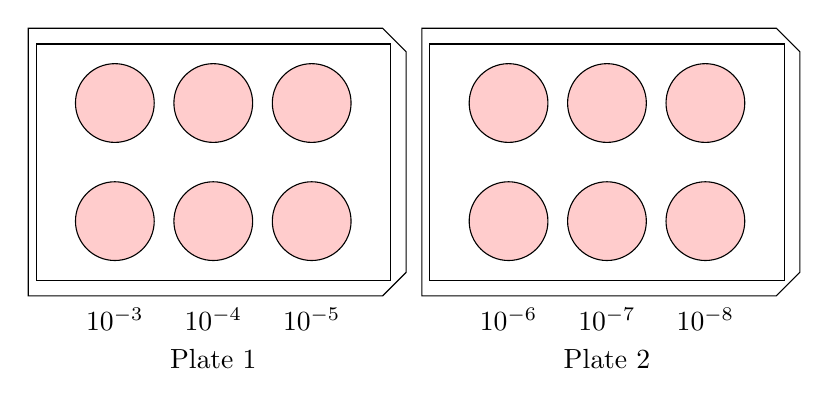
\begin{tikzpicture}

% Plate 1
\draw (0, 0) rectangle (4.5, 3);
\draw (-0.1, -0.2) -- (4.4, -0.2) -- (4.7, 0.1) -- (4.7, 2.9) -- (4.4, 3.2) -- (-0.1, 3.2) -- cycle;

% Wells
\draw [fill=red!20] (1, 0.75) circle (0.5);
\draw [fill=red!20] (1, 2.25) circle (0.5);
\node at (1,-0.5) {$10^{-3}$};

\draw [fill=red!20] (2.25, 0.75) circle (0.5);
\draw [fill=red!20] (2.25, 2.25) circle (0.5);
\node at (2.25,-0.5) {$10^{-4}$};

\draw [fill=red!20] (3.5, 0.75) circle (0.5);
\draw [fill=red!20] (3.5, 2.25) circle (0.5);
\node at (3.5,-0.5) {$10^{-5}$};

\node at (2.25, -1) {Plate 1};

% Plate 2
\draw (5, 0) rectangle (9.5, 3);
\draw (4.9, -0.2) -- (9.4, -0.2) -- (9.7, 0.1) -- (9.7, 2.9) -- (9.4, 3.2) -- (4.9, 3.2) -- cycle;

% Wells
\draw [fill=red!20] (6, 0.75) circle (0.5);
\draw [fill=red!20] (6, 2.25) circle (0.5);
\node at (6,-0.5) {$10^{-6}$};

\draw [fill=red!20] (7.25, 0.75) circle (0.5);
\draw [fill=red!20] (7.25, 2.25) circle (0.5);
\node at (7.25,-0.5) {$10^{-7}$};

\draw [fill=red!20] (8.5, 0.75) circle (0.5);
\draw [fill=red!20] (8.5, 2.25) circle (0.5);
\node at (8.5,-0.5) {$10^{-8}$};

\node at (7.25, -1) {Plate 2};

\end{tikzpicture}
\end{center}

Incubate the plates at $37^{\circ}$C for 1 hour.

Liquify a jar of $1.2\%$ agarose using a microwave. Warm 2x EMEM to $37^{\circ}$C in a water bath. For each plate infected, prepare a solution of 10mL agarose, 10mL 2x EMEM, and $5\mu$L trypsin. (Add the EMEM first, followed by the trypsin, followed by the agarose. Do not add trypsin to hot agarose.)

One plate at a time, aspirate the viral inoculant. (You may use a new pipet for each well or may use one pipet per plate, aspirating from the lowest concentration well to highest.) Quickly add to each well $\sim 3$mL of the agarose solution. Place the lid on the well and allow it to sit, undisturbed, for approximately 30 minutes (or until the agarose overlay has solidified). Incubate for several days at $37^{\circ}$C.

\subsection{Procedure for Performing RV Plaque Assay}

{\bfseries Items Needed:} \begin{enumerate}
	\item Neutral red
	\item 2x EMEM
	\item 1.2\% Agarose
\end{enumerate}

Liquefy 1.2\% agarose by microwave. For 4 6-well plates, mix $15$mL 2x EMEM, $15$mL 1.2\% agarose, and 1.5mL neutral red. Add $1$mL solution to each well and allow it to solidify. Incubate the plates at $37^{\circ}$C and count the plaques that have formed after $4-24$ hours of incubation.

\subsection{Procedure for Transducing MA104 Cells with siRNA-Expressing Lentiviral Vectors}

{\bfseries Items Needed:} \begin{enumerate}
	\item 1000x Polybreen
	\item Lentiviral vector
	\item Non-silencing vector (control)
	\item Complete M199
	\item 0.05\% Trypsin
	\item 1x PBS
	\item Trypan blue
\end{enumerate}

This procedure should be performed when the plated MA104 cells are $70-80\%$ confluent.

Select one well to use for a cell count. Aspirate the cell culture medium from this well. Add $1$mL PBS, spread evenly, and aspirate. Add $500\mu$L trypsin, spread evenly, and aspirate. Add $500\mu$L trypsin, spread evenly, and incubate the plate at $37{^\circ}$C until all cells have detached from the well.

To the well add $1.5$mL complete M199 and mix well. Take $10\mu$L cell mix and combine with $10\mu$L trypan blue. Apply this mixture to a slide and determine the number of cells per mL. Normalize this to the number of cells per well. (I.e., double the cell count per mL for the $2$mL cell soln in the target well.)

Calculate the dilution factor for the lentiviral vector by:
\begin{equation}
\left(\frac{\text{cells}}{\text{well}}\cdot \text{MOI}\right)/\left[\text{lentivirus}\right]
\end{equation}

For example, if there are $1.86\times 10^5$ cells per well, your original lentiviral concentration is $2.13\times 10^9$ particles per mL, and you want to transfect your cells with a multiplicity of infection (MOI) of $10$:
\begin{align*}
\text{dilution} &= \left(\frac{1.86\e{5}\text{ cells}}{\text{well}}\cdot \frac{10\text{ particles}}{1\text{ cell}}\right)/\frac{2.13\e{9}\text{ particles}}{\text{mL}} \\
&= \frac{1.86\e{6}\text{ particles}}{\text{well}}/\frac{2.13\e{9}\text{ particles}}{\text{mL}} \\
&= \frac{0.00087\text{mL}}{\text{well}} = \frac{0.87\mu\text{L}}{\text{well}}
\end{align*}

Per well, prepare a solution of $1$mL complete M199, $1\mu$L polybreen (diluted by a factor of $1000$), and the calculated volume of lentiviral vector. Repeat this procedure for the control NSV.

Aspirate the cell culture medium from each control and experimental well. To the experimental wells, add with one pipet $1$mL lentiviral solution to each well. To the control wells, add with a second pipet $1$mL control solution to each well. The final plates, using $5$ control and $5$ experimental wells, may look similar to the following:

\begin{center}
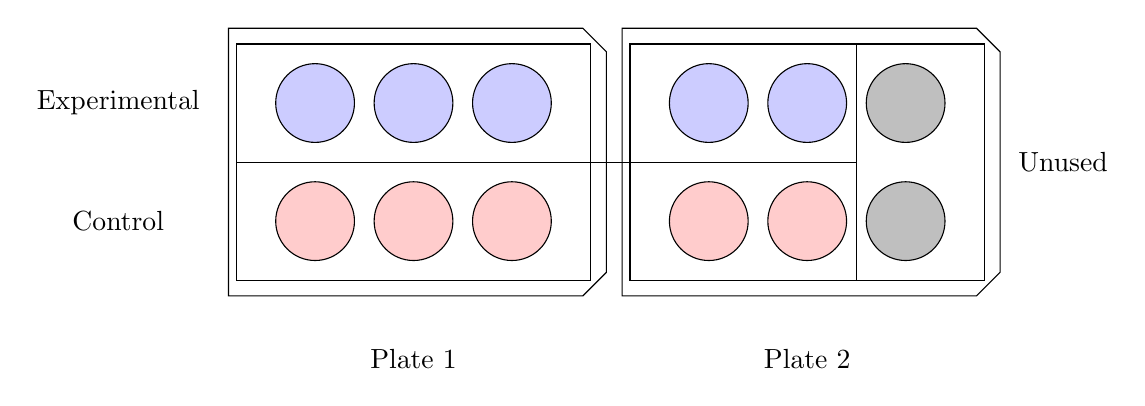
\begin{tikzpicture}

% Plate 1
\draw (0, 0) rectangle (4.5, 3);
\draw (-0.1, -0.2) -- (4.4, -0.2) -- (4.7, 0.1) -- (4.7, 2.9) -- (4.4, 3.2) -- (-0.1, 3.2) -- cycle;

% Wells
\draw [fill=red!20] (1, 0.75) circle (0.5);
\draw [fill=blue!20] (1, 2.25) circle (0.5);

\draw [fill=red!20] (2.25, 0.75) circle (0.5);
\draw [fill=blue!20] (2.25, 2.25) circle (0.5);

\draw [fill=red!20] (3.5, 0.75) circle (0.5);
\draw [fill=blue!20] (3.5, 2.25) circle (0.5);

\node at (2.25, -1) {Plate 1};

% Plate 2
\draw (5, 0) rectangle (9.5, 3);
\draw (4.9, -0.2) -- (9.4, -0.2) -- (9.7, 0.1) -- (9.7, 2.9) -- (9.4, 3.2) -- (4.9, 3.2) -- cycle;

% Wells
\draw [fill=red!20] (6, 0.75) circle (0.5);
\draw [fill=blue!20] (6, 2.25) circle (0.5);

\draw [fill=red!20] (7.25, 0.75) circle (0.5);
\draw [fill=blue!20] (7.25, 2.25) circle (0.5);

\draw [fill=gray!50] (8.5, 0.75) circle (0.5);
\draw [fill=gray!50] (8.5, 2.25) circle (0.5);

\node at (7.25, -1) {Plate 2};

\draw (0, 1.5) -- (7.875, 1.5);
\draw (7.875, 0) -- (7.875, 3);

\node [align = right] at (-1.5, 2.25) {Experimental};
\node [align = right] at (-1.5, 0.75) {Control};
\node at (10.5, 1.5) {Unused};
\end{tikzpicture}
\end{center}

Incubate these plates for 2 hours at $37^{\circ}$C. After 2 hours, add to each of the experimental wells $2$mL complete M199. Using a second pipet, add to each of the control wells $2$mL completeM199. The final volume of medium in each well should be $3$mL. Incubate for 48 hours at $37^{\circ}$C.

\subsection{Procedure for Infecting Cells Following Lentiviral Transduction}

\subsection{Procedure for Cell Count Following Infection of Lentivirally-Transduced Cells}

	\clearpage
	\pagestyle{style2}
	\part{Lab Notes \& Daily Log}
	%%%%%%%%%%
	% August 2014
	%%%%%%%%%%
	\input{logs/2014_08_31.tex}

	%%%%%%%%%%
	% September 2014
	%%%%%%%%%%
	\input{logs/2014_09_07.tex}
	\input{logs/2014_09_14.tex}
	\input{logs/2014_09_21.tex}
	\input{logs/2014_09_28.tex}
	
	%%%%%%%%%%
	% October 2014
	%%%%%%%%%%
	\input{logs/2014_10_05.tex}
	\input{logs/2014_10_12.tex}
	\input{logs/2014_10_19.tex}
	\input{logs/2014_10_26.tex}
	
	%%%%%%%%%%
	% November 2014
	%%%%%%%%%%
	\input{logs/2014_11_02.tex}

\end{document}